%% Based on a TeXnicCenter-Template by Tino Weinkauf.
%%%%%%%%%%%%%%%%%%%%%%%%%%%%%%%%%%%%%%%%%%%%%%%%%%%%%%%%%%%%%

%%%%%%%%%%%%%%%%%%%%%%%%%%%%%%%%%%%%%%%%%%%%%%%%%%%%%%%%%%%%%
%% HEADER
%%%%%%%%%%%%%%%%%%%%%%%%%%%%%%%%%%%%%%%%%%%%%%%%%%%%%%%%%%%%%
\documentclass[a4paper,oneside,10pt]{report}
%\usepackage[cp1250]{inputenc} % jeśli kodowanie edytowanych plików to cp1250 
\usepackage[utf8]{inputenc} % jeśli kodowanie edytowanych plików to UTF8

% Alternative Options:
%	Paper Size: a4paper / a5paper / b5paper / letterpaper / legalpaper / executivepaper
% Duplex: oneside / twoside
% Base Font Size: 10pt / 11pt / 12pt


%% Language %%%%%%%%%%%%%%%%%%%%%%%%%%%%%%%%%%%%%%%%%%%%%%%%%
%\usepackage[T1]{fontenc}
\usepackage[polish]{babel}
\usepackage[OT4]{fontenc}
\usepackage[ansinew]{inputenc}

\usepackage{lmodern} %Type1-font for non-english texts and characters

%% Remove chapte %%%%%%%%%%%%%%%%%%%%%%%%%%%%%%%%%%%%%%%%%%%%
\usepackage{titlesec}
\titleformat{\chapter}[display]
{\normalfont\huge\bfseries}{}{0pt}{\Huge}
\titlespacing*{\chapter} {0pt}{20pt}{40pt}

%% Packages for Graphics & Figures %%%%%%%%%%%%%%%%%%%%%%%%%%
\usepackage{graphicx} %%For loading graphic files
%\usepackage{subfig} %%Subfigures inside a figure
%\usepackage{pst-all} %%PSTricks - not useable with pdfLaTeX

%% Please note:
%% Images can be included using \includegraphics{Dateiname}
%% resp. using the dialog in the Insert menu.
%% 
%% The mode "LaTeX => PDF" allows the following formats:
%%   .jpg  .png  .pdf  .mps
%% 
%% The modes "LaTeX => DVI", "LaTeX => PS" und "LaTeX => PS => PDF"
%% allow the following formats:
%%   .eps  .ps  .bmp  .pict  .pntg

%% Math Packages %%%%%%%%%%%%%%%%%%%%%%%%%%%%%%%%%%%%%%%%%%%%
\usepackage{amsmath}
\usepackage{amsthm}
\usepackage{amsfonts}

%% ASM Packages %%%%%%%%%%%%%%%%%%%%%%%%%%%%%%%%%%%%%%%%%%%%%
\usepackage{listings}
\usepackage{tcolorbox} 
\lstdefinelanguage
   [x64]{Assembler}     % add a "x64" dialect of Assembler
   [x86masm]{Assembler} % based on the "x86masm" dialect
   % with these extra keywords:
   {morekeywords={	movl, pushl,
   				  CDQE,CQO,CMPSQ,CMPXCHG16B,JRCXZ,LODSQ,MOVSXD, %
                  POPFQ,PUSHFQ,SCASQ,STOSQ,IRETQ,RDTSCP,SWAPGS, %
                  rax,rdx,rcx,rbx,rsi,rdi,rsp,rbp, %
                  r8,r8d,r8w,r8b,r9,r9d,r9w,r9b}} % etc.

\lstset{
	language=[x64]Assembler,
    keywordstyle=\color{blue},
    stringstyle=\color{red},
    commentstyle=\color{green},
    morecomment=[l][\color{magenta}]{\#}
}


\usepackage{float}
\usepackage{hyperref}
\usepackage[fixlanguage]{babelbib}


%% Line Spacing %%%%%%%%%%%%%%%%%%%%%%%%%%%%%%%%%%%%%%%%%%%%%
%\usepackage{setspace}
%\singlespacing        %% 1-spacing (default)
%\onehalfspacing       %% 1,5-spacing
%\doublespacing        %% 2-spacing


%% Other Packages %%%%%%%%%%%%%%%%%%%%%%%%%%%%%%%%%%%%%%%%%%%
%\usepackage{a4wide} %%Smaller margins = more text per page.
%\usepackage{fancyhdr} %%Fancy headings
%\usepackage{longtable} %%For tables, that exceed one page


%%%%%%%%%%%%%%%%%%%%%%%%%%%%%%%%%%%%%%%%%%%%%%%%%%%%%%%%%%%%%
%% Remarks
%%%%%%%%%%%%%%%%%%%%%%%%%%%%%%%%%%%%%%%%%%%%%%%%%%%%%%%%%%%%%
%
% TODO:
% 1. Edit the used packages and their options (see above).
% 2. If you want, add a BibTeX-File to the project
%    (e.g., 'literature.bib').
% 3. Happy TeXing!
%
%%%%%%%%%%%%%%%%%%%%%%%%%%%%%%%%%%%%%%%%%%%%%%%%%%%%%%%%%%%%%

%%%%%%%%%%%%%%%%%%%%%%%%%%%%%%%%%%%%%%%%%%%%%%%%%%%%%%%%%%%%%
%% Options / Modifications
%%%%%%%%%%%%%%%%%%%%%%%%%%%%%%%%%%%%%%%%%%%%%%%%%%%%%%%%%%%%%

%\input{options} %You need a file 'options.tex' for this
%% ==> TeXnicCenter supplies some possible option files
%% ==> with its templates (File | New from Template...).



%%%%%%%%%%%%%%%%%%%%%%%%%%%%%%%%%%%%%%%%%%%%%%%%%%%%%%%%%%%%%
%% DOCUMENT
%%%%%%%%%%%%%%%%%%%%%%%%%%%%%%%%%%%%%%%%%%%%%%%%%%%%%%%%%%%%%
\begin{document}
%% Title Page %%%%%%%%%%%%%%%%%%%%%%%%%%%%%%%%%%%%%%%%%%%%%%%
%% ==> Write your text here or include other files.

%% The nice version:
%% Based on a TeXnicCenter-Template by Tino Weinkauf.
%%%%%%%%%%%%%%%%%%%%%%%%%%%%%%%%%%%%%%%%%%%%%%%%%%%%%%%%%%%%%

%%%%%%%%%%%%%%%%%%%%%%%%%%%%%%%%%%%%%%%%%%%%%%%%%%%%%%%%%%%%%
%% Deckblatt
%%%%%%%%%%%%%%%%%%%%%%%%%%%%%%%%%%%%%%%%%%%%%%%%%%%%%%%%%%%%%
%%
%% ATTENTION: You need a main file to use this one here.
%%            Use the command "\input{filename}" in your
%%            main file to include this file.
%%


\begin{titlepage}
\centering
	{\scshape\LARGE Politechnika Wrocławska \par}
	\vspace{6cm}
	{\huge\bfseries Architektura Komputerów 2 - laboratorium\par}
	\vspace{0.5cm}
	{\Large\itshape sprawozdanie\par}
    \vspace{2cm}
    \vfill
	Autor:\par
	~Jarosław \textsc{Piszczała} 209983
	\vfill
	Prowadzący:\par
	Prof. ~Janusz \textsc{Biernat}
	\vfill
   Wydział Elektroniki\par
   Informatyka\par
   IV rok
   \vfill

% Bottom of the page
	{\large \today\par}
\end{titlepage}
%\newpage
%\setcounter{page}{2}

%% The simple version:

 %%You need a file 'titlepage.tex' for this.
%% ==> TeXnicCenter supplies a possible titlepage file
%% ==> with its templates (File | New from Template...).


%% Inhaltsverzeichnis %%%%%%%%%%%%%%%%%%%%%%%%%%%%%%%%%%%%%%%
\tableofcontents %Table of contents
\cleardoublepage %The first chapter should start on an odd page.

%\pagestyle{plain} %Now display headings: headings / fancy / ...



%% Chapters %%%%%%%%%%%%%%%%%%%%%%%%%%%%%%%%%%%%%%%%%%%%%%%%%
%% ==> Write your text here or include other files.

%\input{intro} %You need a file 'intro.tex' for this.


%%%%%%%%%%%%%%%%%%%%%%%%%%%%%%%%%%%%%%%%%%%%%%%%%%%%%%%%%%%%%
%% ==> Some hints are following:


%\chapter{Laboratorium 1}
\section{Tematyka}
Tematem laboratorium było zapoznanie się z podstawowymi działaniami z wykorzystaniem
instrukcji assemblerowych. Głównym celem zajęć było przetwarzanie ciągów znaków.
\section{Zakres prac}
Zadaniem było stworzenie trzech aplikacji.
\begin{enumerate}
	\item Program który zamieniałby, w ciągu znaków, znaki duże na małe oraz małe na duże
	\item Program który implementowałby prosty szyfr cezara
	\item Program który szyfrował i deszyfrowałby liczby całkowite (wykorzystując program z zadania drugiego)
Program szyfrujący miałby zostać stworzony w wariancie 32 oraz 64 bitowym.
\end{enumerate}
\section{Rozwiązanie}
\subsection{Zamienianie znaków}
Pierwsze zadanie nie było trudne. Dzięki obszernej instrukcji do zajęć laboratoryjnych bezproblemowo udało się wykonać ten prosty typ programu. Poniższy kod jest odpowiedzialny za pobranie, zmiane rozmiaru i ponowne zapisanie znaku.
\begin{lstlisting}[frame=single, basicstyle=\small, caption=Funkcja zmieniająca rozmiar znaków]
function:
 movb in(,%esi,1), %al
 cmp $END_OF_LINE, %al
 je end
 cmp $'Z', %al
 jle big
 sub $DISTANCE, %al
 movb %al, out(,%esi,1)
 inc %esi
 jmp function

big:
 add $DISTANCE, %al
 movb %al, out(,%esi,1)
 inc %esi
 jmp function
\end{lstlisting}
Nie jest to najbardziej optymalny typ rozwiązania. Z aktualną wiedzą stwierdzam, że wystarczyłoby na każdej z liter użyć funkcji XOR z odpowiednią maską która zamieniałaby jeden bit na odwrotny, który odpowiada za rozmiar litery. Takie rozwiązanie zostało wprowadzone podczas pisania funkcji XOR'ującej na kolejnych laboratoriach.
\subsection{Szyfr cezara}
Szyfr cezara to jeden z najbardziej znanych typów szyfrowania. Pierwszy znak wyznacza przesunięcie znaków w alfabecie. Przyjęto, iż znak "`A"' oznacza brak szyfrowania. Przyjęto także, że duży pierwszy znak ma powodować szyfrowanie, a mały znak deszyfrowanie. A co dalej następuje, pierwszy znak należy najpierw wyciągnąć i zweryfikować z czym mamy do czynienia.

\begin{lstlisting}[frame=single, basicstyle=\small, caption=Rozpoznanie znaku]
Sign:
 mov $0, %ecx
 movb in(,%esi,1), %cl

 cmp $'A', %cl
 jl end
 cmp $'z', %cl
 jg end
 cmp $'Z', %cl
 jle Decryption

Encryption:
 sub $'a', %ecx
eFunction:
 inc %esi
 movb in(,%esi,1), %al
 cmp $END_OF_LINE, %al
 je end
\end{lstlisting}

Po zapoznaniu się ze znakiem i typu działania, rozpoczynamy działanie na reszcie ciągu znaków. Każdy ze znaków należy przesunąć o odpowiednią wartość w lewo lub prawo, a następnie zweryfikować, czy nie wyszliśmy poza zakres liter. W przypadku przekroczenia zakresu liter, należy odjąć litery, aby doprowadzić do zapętlenia.

\subsection{Szyfrowanie liczb}
Z szyfrowaniem liczb nie było dużego problemu. Postawione założenie mówi, iż gdy w ciągu znaków zostaną odnalezione cyfry, należy je poprzedzić znakiem "`X"', a każdą z cyfr potraktować jak kolejne znaki alfabetu. Dla przykładu dla liczby "`1994"' należałoby przeprowadzić konwersje na "`xAIID"'. Budzi to pewne obawy, gdyż przy dekodowaniu po trafieniu na znak "`X"' powinniśmy znaki z zakresu od A do I traktować jako liczby, a co jeśli to już będzie zakodowana treść a nie liczba? Tak więc do kodu z zadania drugiego została dorobiona funkcja która sprawdza nasz ciąg znaków i w miarę potrzeby zamienia wykryte w nim liczby według powyższego schematy 

\begin{lstlisting}[frame=single, basicstyle=\small, caption=Szyfrowanie liczb całkowitych]
 movb text(,%esi,1), %cl
 cmp $END_OF_LINE, %cl
 je trEnd
 cmp $'0', %cl
 jl trSave
 cmp $'9', %cl
 jg trSave

trNumberStart:
 movb $'X', in(,%edi,1)
 inc %edi

trNumber:
 subb $NUMBER, %cl
 addb $'A', %cl
 movb %cl, in(,%edi,1)
 inc %esi
 inc %edi
\end{lstlisting}

\section{Wnioski}
Pisanie w assemblerze nie jest prostym tematem. Należy zwracać uwagę na wiele szczegółów na które przy pisaniu chociażby w C nikt nie zwraca uwagi. Najtrudniej było rozpocząć pracę z instrukcjami, pamiętać co dzieje się z rejestrami w przypadku niektórych instrukcji. W przypadku pisania aplikacji pod system x86, przy małej ilości rejestrów bardzo pomocny okazał się bufor i stos. Inny problem sprawiło późniejsze zrozumienie co dzieje się w kodzie, gdzie z pomocą przyszedł debugger GDB. Dzięki opanowaniu tego narzędzia z powodzeniem można było przejrzeć krokowo zmiany w pamięci i rejestrze.
%\chapter{Laboratorium 2}
\section{Tematyka}
Tematem laboratorium było zapoznanie się z działaniem stosu i tworzeniem funkcji
go wykorzystujących.
\section{Zakres prac}
Zadaniem było stworzenie trzech aplikacji.
\begin{enumerate}
	\item Program z funkcją do xor'owania liczb
	\item Program z funkcją wykorzystujący pętlę sterującą (np. silnia, fibonacci)
	\item Program z funkcją rekurencyjną (np. silnia, fibonacci)
\end{enumerate}
Programy powinny zostać wykonane w wariancie 32 oraz 64 bitowym. Celem jest możliwość porównania czasu działania, oraz przejrzystości kodu dla dwóch typów pisania funkcji (rekurencyjnej oraz z użyciem pętli)

\section{Rozwiązanie}
\subsection{XOR'orwanie liczb}
Jako pierwsze zadanie, aby zapoznać się ze sposobem tworzenia funkcji i przekazywania argumentów stworzono funkcje xor. Funkcja ta ma stworzoną maskę do zmiany rozmiaru znaków wprowadzanych jako argument funkcji. Ważna jest tutaj przyjęta konwencja, aby argumenty na stos przed wywołaniem funkcji wprowadzać w odwrotnej kolejności. Na początku funkcji zabezpieczamy aktualną wartość rejestru "`ebp"' aby nie utracić adresu powrotu z funkcji. Na końcu przywracamy ten rejestr i używamy instrukcji return która wróci do miejsca gdzie została wywołana funkcja.
\begin{lstlisting}[frame=single, basicstyle=\small, caption=Funkcja XORująca]
 push %eax
 call xor_func
 pop %ecx

 mov $EXIT, %eax
 mov $ERROR, %ebx
 int $SYSCALL

xor_func:
 push %ebp
 mov %esp, %ebp
 mov 8(%ebp),%ebx
 
 xor $0b00100000, %ebx

 mov %ebx, 8(%ebp)
 mov %ebp, %esp
 pop %ebp
 ret
\end{lstlisting}

\subsection{Silnia wykorzystująca rekurencje}
Funkcja rekurencyjna powinna być tak zaprojektowana, aby wywoływać samą siebie w przypadku gdy nie zostanie spełniona pewna własność. W przypadku silni, uruchamiamy kolejną funkcje dopóki nie zejdziemy do pierwszej liczby. Większość kodu funkcji rekurencyjnej to wprowadzanie argumentów, ich odczyt, i wywoływanie funkcji.
\begin{lstlisting}[frame=single, basicstyle=\small, caption=Silnia - rekurencyjnie]
Silnia:
 push %ebp
 mov %esp, %ebp
 mov 8(%ebp), %eax
 cmp $1, %eax
 je EndSilnia
 dec %eax
 push %eax
 call Silnia
 mov 8(%ebp), %ebx
 mul %ebx
EndSilnia:
 mov %ebp, %esp
 pop %ebp
 ret
\end{lstlisting}

Dla porównania ilości kodu oraz jego skomplikowania, została napisana silnia iteracyjna. Jest dużo prostsza, gdyż od razu przechodzi do liczenia, i wymnaża kolejne wartości aż do momentu gdy mnożnik będzie równy wprowadzonemu jako argument funkcjii.
\begin{lstlisting}[frame=single, basicstyle=\small, caption=Silnia - iteracyjnie]
 mov $1, %eax
 mov $0, %ecx
Silnia:
 inc %ecx
 mul %ecx
 cmp %ebx, %ecx
 jne Silnia
\end{lstlisting}
Jak widać, silnia iteracyjna jest dużo prostsza w zapisie i łatwiejsza do czytania niż jej wersja rekurencyjna. Jest też dużo mniej awaryjna, gdyż jest mniejsza szansa na utracenie danych.
\section{Wnioski}
Pisanie funkcji w assemblerze jest podobne do pisania funkcji w C. Oczywiście nie jest ono dokładnie tak samo, gdyż wymaga od nas pamiętania o wielu szczegółach takich jak kolejność wprowadzania wartości na stos, czy zapamiętanie adresu powrotu. Mimo wszystko pisanie funkcji nie jest trudne. 
%\chapter{Laboratorium 3}
\section{Tematyka}
Tematem laboratorium było zapoznanie się ze sposobem łączenia instrukcji assemblerowych
z kodem napisanym w C.
\section{Zakres prac}
Zadaniem było stworzenie trzech aplikacji wykorzystując łączenie asemblera z C:
\begin{enumerate}
	\item Program który wczyta dane w C, przetworzy je w ASM a następnie wyświetli w C
	\item Program który wczyta dane w ASM, przetworzy i wyświetli w C
	\item Program który wczyta dane w C, przetworzy je za pomocą wstawki ASM a następnie wyświetli w C
\end{enumerate}}

\section{Rozwiązanie}
Od strony C zadanie nie wymagało dużej wiedzy. Aby skorzystać z funkcji napisanej w ASM należało dodać tutaj regułkę "`extern"'. Dzięki temu już mogliśmy działać z naszą funkcją, a jeśli wystąpiłby błąd - były on spowodowany na pewno po stronie kodu ASM.
\begin{lstlisting}[language=c, frame=single,showstringspaces=false, basicstyle=\small, caption=Funkcja obliczająca silnie iteracyjnie]
#include <stdio.h>

extern int silnia(int num);

int main(){
	int wartosc;
	scanf("%d", &wartosc);
	int wynik = silnia(wartosc);
	printf("Silnia z %d = %d\n",wartosc, wynik);
}
\end{lstlisting}

Do połączenia wykorzystano funkcję z poprzednich zajęć do obliczania iteracyjnie silni.

\begin{lstlisting}[frame=single, basicstyle=\small, caption=Funkcja obliczająca silnie iteracyjnie]
.text
.globl silnia
silnia:
 pushq %rbp
 movq %rsp, %rbp
 movq %rdi, %rbx  
 
 mov $1, %eax
 mov $0, %ecx
Silnia_func:
 inc %ecx
 mul %ecx
 cmp %ebx, %ecx
 jne Silnia_func

 movq %rbp, %rsp
 pop %rbp
ret
\end{lstlisting}

Ze względu na problemy przy kompilacji oraz problem niedoczytania dokumentacji kompilatora, nie udało się wykonać na zajęciach więcej zadań. Na sprzęcie laboratoryjnym brakowało biblioteki do kompilacji kodu 32 bitowego, przez co należało przejść na kod 64 bitowy. Ten natomiast przy kompilacji za pomocą "`gcc"' nie wprowadzał pierwszych 6 argumentów na stos, a do rejestrów. Z tego kompilatora wycofano opcje dodania flagi, aby argumenty trafiły na stos.

\section{Wnioski}
Łączenie języków C i assembler przebiega w dużej mierze bezkolizyjnie. Może się to przydać w sytuacji gdy chcemy wykorzystać w naszym kodzie assemblerowym jakąś funkcję napisaną w C, której nie chcemy przepisywać na assemblera bądź gdy chcemy przyspieszyć pewne operacje poprzez wykonanie operacji za pomocą instrukcji assemblerowych. Problem zaczyna się, gdy chcemy przenieść się na platformę 64 bitową, gdyż nowa wersja "`gcc"' nie wspiera wprowadzania wszystkich argumentów na stos, przez co kod wymaga dużo większej refaktoryzacji.
%\chapter{Laboratorium 4}

\section{Tematyka}
Tematem laboratorium było zapoznanie się z działaniem FPU.
\section{Zakres prac}
Zadaniem było stworzenie trzech aplikacji wykorzystujących łączenie ASM i C:
\begin{enumerate}
	\item Program który odczyta i zinterpretuje dane z rejestru stanu (FPSR) oraz ustawi odpowiednie bity rejestru sterującego (FPCR)
	\item Program który wytwarza poszczególne wyjątki zmiennoprzecinkowe i wyświetla odpowiednie komentarze
	\item Program który pozwoli na przeprowadzenie operacji zmiennoprzecinkowych w dwóch wersjach. Pierwsza jako proste liczenie pola trójkąta, druga wykorzystująca iteracje (np. metoda Newtona-Raphsona)
\end{enumerate}
Przy każdym z zadań działania powinny być przeprowadzone w kodzie ASM. Cała reszta jak pobranie argumentów czy wyświetlenie wyników powinno być wykonane w C.

\section{Rozwiązanie}
\subsection{Odczytanie rejestru stanu}
Do odczytania rejestru stanu wykorzystano specjalne instrukcje. Następnie po uzyskaniu wartości statusu, należało zweryfikować jego poszczególne bity. Nas interesowało pierwsze sześć bitów. Aby tego dokonać w jak najprostszy sposób skorzystano z intrukcji "`shr"' która przesuwa bity o zadaną ilość bitów w prawo, przy przesuwaniu ich o jeden bit, ten trafiał do flagi TODO (flagi przeniesienia), a tą można zweryfikować instrukcją "`lea"'. W ten sposób sprawdzono każdy kolejny bit, i wyświetlono odpowiedni komunikat gdy natrafiono na przeniesienie.
\begin{lstlisting}[frame=single, basicstyle=\small, caption=Odczytanie i weryfikacja rejestru stanu]
  fstsw	statusword
  fwait
  mov	statusword, %bx

  mov $1, %cl
  and $0, %rax
check_operation:
  shr %rbx
  jnc check_denormal
  leaq err_operation, %rdi
  call printf
\end{lstlisting}
Ze względu na dopieszczenie kodu do perfekcji, zmieniając metody przetwarzania statusu, to zadanie zajęło zbyt dużą część laboratorium. Odczytanie rejestru sterującego byłoby rozwiązane w sposób podobny, jednakże tam uwagę należałoby zwrócić na dwie pary bitów: 11-10 oraz 9-8. Bity sprawdzamy tak jak powyżej, z pomocą instrukcji "`shr"'. 

\section{Wnioski}
Ze względu na problemy związane ze zrozumieniem działania jednostki zmiennoprzecinkowej oraz problemu związanego z pewnymi instrukcjami na zajęciach laboratoryjnych nie udało się ukończyć drugiej części zadania. Jest to na pewno jednostka bardzo przydatna do przeprowadzania dokładnych obliczeń, z wartościami po przecinku. Pisanie kodu w assemblerze pozwala nam także na zmianę precyzji tych obliczeń oraz sposobu zaokrąglania co także można uznać za plus.

%\chapter{Laboratorium 5}
\section{Wstęp teoretyczny}
\subsection{Format BMP}
Format BMP został stworzony do grafiki bitmapowej\cite{bmp}. W strukturę tego formatu wchodzi nagłówek oraz tabela pikseli. W nagłówku zapisane są wszelkie informacje na temat charakterystyki bitmapy z których najważniejsze to: wysokość, szerokość, oraz liczba bitów na piksel. Jest to istotne, gdyż te wartości wpływają na budowę tabeli pikseli [Rysunek {\ref{fig:BMP}]. Istotna jest także jej budowa, gdyż tabela pikseli jest zapisana od dołu do góry, od lewej do prawej. Oznacza to, iż dolny lewy róg jest jej początkiem, a prawy góry róg - końcem. Ważny jest też \textit{padding}, gdyż w strukturze ilość bajtów w każdym wierszu musi być potęgą liczby 4.

\begin{figure}[H]
\centering
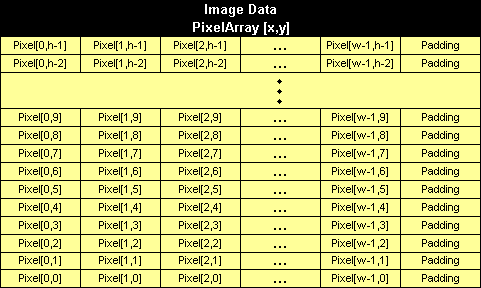
\includegraphics[height=6cm]{images/bmp.png}
\caption{tabela pikseli}
\label{fig:BMP}
\end{figure}

\subsection{Architektura MMX}
Jest ona wykorzystywana głównie przetwarzania dużych ilości danych gdzie wykorzystywany jest jeden algorytm. Najważniejszymi cechami tejże architektury są\cite{userguide}:
\begin{itemize}
\item 8 rejestrów 64 bitowych wykorzystujących rejestry FPU (MM0 - MM7).
\item typ danych "packed". Jego działanie polega na traktowaniu rejestru 64 bitowego jako wektora pewnej liczby komórek o tej samej wielkości.
\item format instrukcji. Instrukcje dla MMX budowane są w kolejności: \textbf{P}, skrót rozkazu/instrukcja (np. \textbf{ADD}), litery \textbf{S} dla wartości ze znakiem bądź \textbf{U} dla wartości bez znaku, \textbf{S} jeśli operacja jest wykonywana z nasyceniem, litery \textbf{L} lub \textbf{H} jeśli operacja wykonywana jest na mniej lub bardziej znaczących bitach oraz \textbf{B}, \textbf{W}, \textbf{D}, \textbf{Q} które odpowiadają za rozmiar komórki wektora. Przykładowa instrukcja MMX: \textbf{PADDUSB} (równoległe dodawanie, bez znaku z saturacją, bajtów).
\end{itemize}
\section{Zakres prac}
Zadaniem było stworzenie programu w C który wczytywał by plik graficzny (bmp, jpg) i wprowadzałby na nim filtry (odbicia poziome, pionowe oraz po przekątnej, saturacja, negatyw). Następnie należało wybrany filtr napisać w ASM, i porównać czas działania funkcji w C i ASM.
\section{Rozwiązanie}
Do stworzenia funkcji w C można było wykorzystać gotowy schemat ze strony \textit{Zakładu Architektury Komputerów}\cite{zak} który potrafił wczytać oraz zapisać pliki graficzne. Przed przystąpieniem do tworzenia filtrów zostały do kodu programu dodane dwie zmienne (\ref{l:zmienne}): \textit{rowSize} odpowiedzialne za długość wiersza w tablicy pikseli oraz \textit{padding} będące wartością paddingu w aktualnie wczytanym pliku. 

\begin{lstlisting}[language=C, frame=single, caption=Dodatkowe zmienne , label=l:zmienne, basicstyle=\small]  
int rowSize = 
	(( image->format->BitsPerPixel * image->w + 31) / 32) * 4;
int padding = 
	4 - ( (image->w * image->format->BytesPerPixel) % 4);
\end{lstlisting}

\subsection{Operacje na tabeli pikseli}
Przestawianie pikseli w tablicy pikseli należy do trudniejszych zadań. Należy pamiętać o kolejności wierszy w pliku, nie można zapomnieć o występowaniu paddingu co utrudnia operacje przeprowadzane za pomocą prostych pętli for, poza tym działamy na macierzy jednowymiarowej interpretowanej później jako macierz dwuwymiarowa. Dla przykładu kod w \ref{l:vertical} przedstawia prostszą funkcję zmieniającą kolejność pikseli. W tym przypadku nie potrzebna nam była wartość \textit{paddingu}. Jest to prosta suma pętli która zamienia piksele miejscami. W poziomie zakres jest od 0 do wartości \textit{rowSize}. Dużo trudniejsze było napisanie funkcji która odbijała by obraz po przekątnej (\ref{l:diagonal}). Przydała się tam wartość \textit{paddingu} dzięki której można było w szybki sposób ograniczać działanie na tablicy.
Najistotniejsze jednakże jest to, aby przenosić wartości pełnych pikseli, a nie wyłącznie kolejne bajty, gdyż wtedy możemy zakłócić kolory poszczególnych pikseli.
\newpage
\begin{lstlisting}[language=C, frame=single, caption=Funkcja odbijająca obraz w pionie , label=l:vertical, basicstyle=\small]  
void verticalFilter(unsigned char * buf, int width,
		int height,int size,char bpp, int rowSize)
{
  int i, j, k;
  char temp;
    for(i=0; i < (height/2) ; i++)
    {
      for(j=0; j < (width*bpp); j++)
      {
        temp = buf[(i *rowSize) +j];
        buf[ (i *rowSize) +j] = buf[ ((height-i-1) *rowSize) +j ];
        buf[ ((height-i-1) *rowSize) +j ] = temp;
      }
    }
}
\end{lstlisting}

\begin{lstlisting}[language=C, frame=single, caption=Funkcja odbijająca obraz po przekątnej , label=l:diagonal, basicstyle=\small]  
void diagonalFilter(unsigned char * buf, int width,
	int height,int size,char bpp, int RowSize, int Padding)
{
  int i, j, k;
  char temp;
  for(i=0; i < height/2; i++)
  {
    for(j=0; j < (width); j++)
    {
      for(k=0; k<bpp; k++)
      {
        temp = buf[ ( i *(RowSize) ) + ( j *bpp ) +k ];
        
        buf[ ( i * RowSize) ) +( j *bpp ) +k ] = buf[ ( (height-
        i) * (RowSize) - Padding ) - ( j * bpp ) + k ];
        
        buf[ ( (height-i) *(RowSize) -Padding ) - 
        ( j *bpp ) +k ] = temp;
      }
    }
  }
}
\end{lstlisting}

\subsection{Operacje na wartościach pikseli}
Dużo łatwiejsze jest przeprowadzanie tej samej operacji na wartościach pikseli. W przypadku negatywu (\ref{l:negat}) sprawa wygląda dość prosto. Wystarczy zanegować wartości każdego bajta, i w ten sposób otrzymujemy obraz w negatywie. Operacje na poszczególnych pikselach są o tyle łatwiejsze, że uruchamiamy odpowiednio przygotowany algorytm na każdym kolejnym wektorze bajtów, bez potrzeby zastanawiania się jak są one rozmieszczone w tabeli pikseli.
\begin{lstlisting}[language=C, frame=single, caption=Funkcja odbijająca obraz w pionie , label=l:negat, basicstyle=\small]  
void negativeFilter(unsigned char * buf, int width,
		int height,int size,char bpp, int RowSize)
{
  int i, j, k;
  char temp;
  for(i=0; i < height ; i++)
  {
    for(j=0; j < (width*bpp); j++)
    {
      buf[ (i*RowSize) + j] = (~buf[ (i*RowSize) + j]);
    }
  }
}
\end{lstlisting}

\section{Wnioski}
Laboratorium nauczyło mnie jak zbudowane są pliki graficzne. Pozwoliło to także zrozumieć sposób w jaki działają programy graficzne, jak działają filtry czy rysowanie. Zapewne po utworzeniu funkcji która konwertowałaby wektor jednowymiarowy w dwuwymiarowy, praca nad filtrami była by dużo prostsza a i kod byłby dużo prostszy w czytaniu. Niestety ze względu na trudność w początkowym zrozumieniu pracy nad tablicą trójwymiarową zapisaną jako wektor jednowymiarowy nie udało się podczas zajęć laboratoryjnych stworzyć kodu w ASM a także porównać czas działania. Mogę wyłącznie przewidywać, że czas działania będzie przynajmniej kilka razy większy ze względu na możliwość działania na kilku wartościach jednocześnie, co podobne w działaniu jest do pracy na wątkach.
\chapter{Laboratorium 6}
\section{Tematyka}
Tematem laboratorium było zapoznanie się z procesorem: wyłuskiwaniem informacji na jego temat, wykorzystywaniem cykli procesora oraz weryfikowania działania pamięci cache.
\section{Zakres prac}
Zadaniem było zapoznanie się z:
\begin{enumerate}
	\item CPUID - Wydobycie informacji na temat procesora i pamięci podręcznej.
	\item RDTSC - Odczyt aktualnego licznika cykli procesora.
	\item CACHE - Instrukcje z rozszerzeniem *"'FENCE"' a także wykonanie pętli z cyklicznym dostępem do kolejnych komórek tablicy.
\end{enumerate}
\section{Rozwiązanie}
\subsection{CPUID}
CPUID pozwala na odczytanie wielu informacji na temat procesora, są to przede wszystkim informacje na temat tego jakie instrukcje on obsługuje czy jakiego rozmiaru posiada pamięć cache i tym podobne. Dostać się do tych informacji można na dwa sposoby które w sumie sprowadzają się do jednego. Pierwszym sposobem jest wprowadzenie "`ID"' do rejestru "`EAX"' i wywołanie funkcji CPUID która zwróci odpowiednie dane do rejestrów EAX-EDX. 
\begin{lstlisting}[frame=single, basicstyle=\small, caption=Funkcja CPUID]
 mov $2, %eax
 cpuid
\end{lstlisting}

Drugim sposobem jest wykorzystanie w C funkcji "`\_\_get\_cpuid"' znajdującej się w bibliotece "`cpuid.h"'. Należy do niej wprowadzić "`ID"' oraz adresy do czterech zmiennych int które będą emulować nasze cztery rejestry.
\begin{lstlisting}[language=C, frame=single, caption=Funkcja odczytująca i weryfikująca cpuid, label=l:vertical, basicstyle=\small]  
#include <cpuid.h>
int main()
{
 int a,b,c,d,lvl;
 lvl = 1;
 __get_cpuid(lvl,&a,&b,&c,&d);
 printf("Floating-point unit on-Chip: %d\n", d & 0x1);
 printf("Intel Architecture MMX technology supported: %d\n", d>>23 & 0x1);
 printf("Streaming SIMD Extensions supported: %d\n", d>>25 & 0x1);
 printf("Streaming SIMD 2 Extensions supported: %d\n", d>>26 & 0x1);
 printf("CLFLUSH line size: %d\n", b>>8 & 0xF);
\end{lstlisting}
Tak jak wspomniano wcześniej, zasada działania jest tak naprawdę taka sama. W wyniku otrzymujemy ciągi 32 bitów które dla odpowiednich "`ID"' mają odpowiednie wartości. Dla przykładu w powyższym kodzie widać, iż dla jedynki możemy wyciągnąć informacje na temat wspieranych technologii, używanych na poprzednich laboratoriach.

\subsection{RDTSC}
Rdtsc jest funkcją która zwraca ilość cykli procesora. W ten sposób najefektywniej można porównywać czas pracy funkcji, algorytmów itp. rozwiązań. Wystarczy odczytać stan procesora przed funkcją, po funkcji i odjąć wartości aby otrzymać ilość cykli procesora potrzebną na wykonanie danego zadania. Na te potrzeby został stworzony poniższy kod asemblerowy aby otrzymywać informacje z RDTSC.
\begin{lstlisting}[frame=single, basicstyle=\small, caption=Funkcja RDTSC]
.global _rdtsc
_rdtsc:
 pushq %rbp
 movq %rsp, %rbp

 rdtsc

 movq %rbp, %rsp
 pop %rbp
ret
\end{lstlisting}

\subsection{Cache}
Pamięć cache pozwala na szybszy dostęp do danych. Gdy tylko procesor widzi, że pracujemy na tablicy, stara się przetrzymywać ją całą w pamięci aby umożliwić jak najszybsze przeprowadzanie operacji. Aby sprawdzić czy to prawda przeprowadzono eksperyment. Do testu stworzono kilka tablic o rozmiarach od dużo mniejszych do dużo większych od rozmiaru cache a także tablice która jest minimalnie od niego większa. Następnie puszczono operacje odczytu z tablicy taką samą ilość razy dla każdej z nich
\begin{lstlisting}[language=C, frame=single, caption=Przykładowa funkcja obliczająca ilość cykli dla odczytu danych z tablicy 4096 intów, label=l:vertical, basicstyle=\small]  
int tablica[4096];
unsigned long start, stop;
int loop=100000;
start = _rdtsc();
for(i=0;i<loop;i++){
	tablica[i%4096];}	
stop = _rdtsc();
printf("Time for 4096 bytes:	%lu\n",stop-start);
\end{lstlisting}
Z tego eksperymentu wynikło, że dla tablic które mieściły się w pamięci cache, czas odczytu wahał się w okolicach podobnej ilości cykli. Dla tablicy która była niewiele większa odnotowano najdłuższy czas dostępu, a dla kolejnych były to ilości pomiędzy poprzednimi wartościami.

\section{Wnioski}
Dzięki laboratorium zapoznano się z działaniem pamięci cache, sposobem testowania czasu działania algorytmów oraz odczytywania danych z procesora. Jest to przydatna wiedza, gdyż pozwoli usprawnić sposób pisania aplikacji, weryfikowania czasu ich działania. Najfajniejsza okazała się funkcja CPUID dzięki której możemy tworzyć aplikacje które same odczytają istotniejsze informacje o naszym procesorze i wykorzystają jego maksymalne możliwości.

\addcontentsline{toc}{section}{\lstlistlistingname}
\lstlistoflistings

%\begin{thebibliography}{9}
%\selectbiblanguage{polish}

%\bibitem{bmp} 
%Strona internetowa:\\
%\url{https://en.wikipedia.org/wiki/BMP\_file\_format} \newline dostęp \today.\\

%\bibitem{userguide} 
%\textit{IA-32 Intel Architecture Software Developer's Manual}\\ \[dostępny w wersji elektronicznej: \url{http://zak.ict.pwr.wroc.pl/materials/architektura/laboratorium/Dokumentacja/Intel\%20Penium\%20IV/}\]. \\

%\bibitem{zak}
%Strona internetowa:
%\url{http://zak.ict.pwr.wroc.pl/materials/architektura/laboratorium/MMX/} \[dostęp \today\].\\

%\end{thebibliography}

%% <== End of hints
%%%%%%%%%%%%%%%%%%%%%%%%%%%%%%%%%%%%%%%%%%%%%%%%%%%%%%%%%%%%%



%%%%%%%%%%%%%%%%%%%%%%%%%%%%%%%%%%%%%%%%%%%%%%%%%%%%%%%%%%%%%
%% BIBLIOGRAPHY AND OTHER LISTS
%%%%%%%%%%%%%%%%%%%%%%%%%%%%%%%%%%%%%%%%%%%%%%%%%%%%%%%%%%%%%
%% A small distance to the other stuff in the table of contents (toc)
%%%\addtocontents{toc}{\protect\vspace*{\baselineskip}}

%% The Bibliography
%% ==> You need a file 'literature.bib' for this.
%% ==> You need to run BibTeX for this (Project | Properties... | Uses BibTeX)
%%%\addcontentsline{toc}{chapter}{Bibliografia} %'Bibliography' into toc
%%%\nocite{*} %Even non-cited BibTeX-Entries will be shown.
%%%\bibliographystyle{plain} %Style of Bibliography: plain / apalike / amsalpha / ...
%%%\bibliography{literature} %You need a file 'literature.bib' for this.

%% The List of Figures
%\clearpage
%\addcontentsline{toc}{chapter}{List of Figures}
%\listoffigures

%% The List of Tables
%\clearpage
%\addcontentsline{toc}{chapter}{List of Tables}
%\listoftables


%%%%%%%%%%%%%%%%%%%%%%%%%%%%%%%%%%%%%%%%%%%%%%%%%%%%%%%%%%%%%
%% APPENDICES
%%%%%%%%%%%%%%%%%%%%%%%%%%%%%%%%%%%%%%%%%%%%%%%%%%%%%%%%%%%%%
\appendix
%% ==> Write your text here or include other files.

%\input{FileName} %You need a file 'FileName.tex' for this.


\end{document}

